\documentclass[twoside]{book}

% Packages required by doxygen
\usepackage{calc}
\usepackage{doxygen}
\usepackage{graphicx}
\usepackage[utf8]{inputenc}
\usepackage{makeidx}
\usepackage{multicol}
\usepackage{multirow}
\usepackage{fixltx2e}
\PassOptionsToPackage{warn}{textcomp}
\usepackage{textcomp}
\usepackage[nointegrals]{wasysym}
\usepackage[table]{xcolor}

% Font selection
\usepackage[T1]{fontenc}
\usepackage{mathptmx}
\usepackage[scaled=.90]{helvet}
\usepackage{courier}
\usepackage{amssymb}
\usepackage{sectsty}
\renewcommand{\familydefault}{\sfdefault}
\allsectionsfont{%
  \fontseries{bc}\selectfont%
  \color{darkgray}%
}
\renewcommand{\DoxyLabelFont}{%
  \fontseries{bc}\selectfont%
  \color{darkgray}%
}
\newcommand{\+}{\discretionary{\mbox{\scriptsize$\hookleftarrow$}}{}{}}

% Page & text layout
\usepackage{geometry}
\geometry{%
  a4paper,%
  top=2.5cm,%
  bottom=2.5cm,%
  left=2.5cm,%
  right=2.5cm%
}
\tolerance=750
\hfuzz=15pt
\hbadness=750
\setlength{\emergencystretch}{15pt}
\setlength{\parindent}{0cm}
\setlength{\parskip}{0.2cm}
\makeatletter
\renewcommand{\paragraph}{%
  \@startsection{paragraph}{4}{0ex}{-1.0ex}{1.0ex}{%
    \normalfont\normalsize\bfseries\SS@parafont%
  }%
}
\renewcommand{\subparagraph}{%
  \@startsection{subparagraph}{5}{0ex}{-1.0ex}{1.0ex}{%
    \normalfont\normalsize\bfseries\SS@subparafont%
  }%
}
\makeatother

% Headers & footers
\usepackage{fancyhdr}
\pagestyle{fancyplain}
\fancyhead[LE]{\fancyplain{}{\bfseries\thepage}}
\fancyhead[CE]{\fancyplain{}{}}
\fancyhead[RE]{\fancyplain{}{\bfseries\leftmark}}
\fancyhead[LO]{\fancyplain{}{\bfseries\rightmark}}
\fancyhead[CO]{\fancyplain{}{}}
\fancyhead[RO]{\fancyplain{}{\bfseries\thepage}}
\fancyfoot[LE]{\fancyplain{}{}}
\fancyfoot[CE]{\fancyplain{}{}}
\fancyfoot[RE]{\fancyplain{}{\bfseries\scriptsize Generated on Tue Aug 19 2014 15\+:23\+:37 for My Project by Doxygen }}
\fancyfoot[LO]{\fancyplain{}{\bfseries\scriptsize Generated on Tue Aug 19 2014 15\+:23\+:37 for My Project by Doxygen }}
\fancyfoot[CO]{\fancyplain{}{}}
\fancyfoot[RO]{\fancyplain{}{}}
\renewcommand{\footrulewidth}{0.4pt}
\renewcommand{\chaptermark}[1]{%
  \markboth{#1}{}%
}
\renewcommand{\sectionmark}[1]{%
  \markright{\thesection\ #1}%
}

% Indices & bibliography
\usepackage{natbib}
\usepackage[titles]{tocloft}
\setcounter{tocdepth}{3}
\setcounter{secnumdepth}{5}
\makeindex

% Hyperlinks (required, but should be loaded last)
\usepackage{ifpdf}
\ifpdf
  \usepackage[pdftex,pagebackref=true]{hyperref}
\else
  \usepackage[ps2pdf,pagebackref=true]{hyperref}
\fi
\hypersetup{%
  colorlinks=true,%
  linkcolor=blue,%
  citecolor=blue,%
  unicode%
}

% Custom commands
\newcommand{\clearemptydoublepage}{%
  \newpage{\pagestyle{empty}\cleardoublepage}%
}


%===== C O N T E N T S =====

\begin{document}

% Titlepage & ToC
\hypersetup{pageanchor=false,
             bookmarks=true,
             bookmarksnumbered=true,
             pdfencoding=unicode
            }
\pagenumbering{roman}
\begin{titlepage}
\vspace*{7cm}
\begin{center}%
{\Large My Project }\\
\vspace*{1cm}
{\large Generated by Doxygen 1.8.7}\\
\vspace*{0.5cm}
{\small Tue Aug 19 2014 15:23:37}\\
\end{center}
\end{titlepage}
\clearemptydoublepage
\tableofcontents
\clearemptydoublepage
\pagenumbering{arabic}
\hypersetup{pageanchor=true}

%--- Begin generated contents ---
\chapter{Hierarchical Index}
\section{Class Hierarchy}
This inheritance list is sorted roughly, but not completely, alphabetically\+:\begin{DoxyCompactList}
\item \contentsline{section}{suker\+R\+D\+A.\+rda\+Pkg.\+suker\+R\+D\+A\+Body.\+abstractor\+Body}{\pageref{classsuker_r_d_a_1_1rda_pkg_1_1suker_r_d_a_body_1_1abstractor_body}}{}
\item Dialog\begin{DoxyCompactList}
\item \contentsline{section}{suker\+R\+D\+A.\+rda\+Pkg.\+suker\+R\+D\+A\+Help.\+Help\+About\+Dialog}{\pageref{classsuker_r_d_a_1_1rda_pkg_1_1suker_r_d_a_help_1_1_help_about_dialog}}{}
\end{DoxyCompactList}
\item Frame\begin{DoxyCompactList}
\item \contentsline{section}{suker\+R\+D\+A.\+rda\+Pkg.\+suker\+R\+D\+A\+Main.\+Abstractor\+Shell}{\pageref{classsuker_r_d_a_1_1rda_pkg_1_1suker_r_d_a_main_1_1_abstractor_shell}}{}
\end{DoxyCompactList}
\item \contentsline{section}{suker\+R\+D\+A.\+rda\+Pkg.\+suker\+R\+D\+A\+Log\+Out.\+log\+Outputs}{\pageref{classsuker_r_d_a_1_1rda_pkg_1_1suker_r_d_a_log_out_1_1log_outputs}}{}
\end{DoxyCompactList}

\chapter{Class Index}
\section{Class List}
Here are the classes, structs, unions and interfaces with brief descriptions\+:\begin{DoxyCompactList}
\item\contentsline{section}{\hyperlink{classsuker_r_d_a_1_1rda_pkg_1_1suker_r_d_a_body_1_1abstractor_body}{suker\+R\+D\+A.\+rda\+Pkg.\+suker\+R\+D\+A\+Body.\+abstractor\+Body} }{\pageref{classsuker_r_d_a_1_1rda_pkg_1_1suker_r_d_a_body_1_1abstractor_body}}{}
\item\contentsline{section}{\hyperlink{classsuker_r_d_a_1_1rda_pkg_1_1suker_r_d_a_main_1_1_abstractor_shell}{suker\+R\+D\+A.\+rda\+Pkg.\+suker\+R\+D\+A\+Main.\+Abstractor\+Shell} }{\pageref{classsuker_r_d_a_1_1rda_pkg_1_1suker_r_d_a_main_1_1_abstractor_shell}}{}
\item\contentsline{section}{\hyperlink{classsuker_r_d_a_1_1rda_pkg_1_1suker_r_d_a_help_1_1_help_about_dialog}{suker\+R\+D\+A.\+rda\+Pkg.\+suker\+R\+D\+A\+Help.\+Help\+About\+Dialog} }{\pageref{classsuker_r_d_a_1_1rda_pkg_1_1suker_r_d_a_help_1_1_help_about_dialog}}{}
\item\contentsline{section}{\hyperlink{classsuker_r_d_a_1_1rda_pkg_1_1suker_r_d_a_log_out_1_1log_outputs}{suker\+R\+D\+A.\+rda\+Pkg.\+suker\+R\+D\+A\+Log\+Out.\+log\+Outputs} }{\pageref{classsuker_r_d_a_1_1rda_pkg_1_1suker_r_d_a_log_out_1_1log_outputs}}{}
\end{DoxyCompactList}

\chapter{Class Documentation}
\hypertarget{classsuker_r_d_a_1_1rda_pkg_1_1suker_r_d_a_body_1_1abstractor_body}{\section{suker\+R\+D\+A.\+rda\+Pkg.\+suker\+R\+D\+A\+Body.\+abstractor\+Body Class Reference}
\label{classsuker_r_d_a_1_1rda_pkg_1_1suker_r_d_a_body_1_1abstractor_body}\index{suker\+R\+D\+A.\+rda\+Pkg.\+suker\+R\+D\+A\+Body.\+abstractor\+Body@{suker\+R\+D\+A.\+rda\+Pkg.\+suker\+R\+D\+A\+Body.\+abstractor\+Body}}
}
\subsection*{Public Member Functions}
\begin{DoxyCompactItemize}
\item 
\hypertarget{classsuker_r_d_a_1_1rda_pkg_1_1suker_r_d_a_body_1_1abstractor_body_ac1b0f6563aa0f47587e4b097d94e9e71}{def {\bfseries \+\_\+\+\_\+init\+\_\+\+\_\+}}\label{classsuker_r_d_a_1_1rda_pkg_1_1suker_r_d_a_body_1_1abstractor_body_ac1b0f6563aa0f47587e4b097d94e9e71}

\item 
\hypertarget{classsuker_r_d_a_1_1rda_pkg_1_1suker_r_d_a_body_1_1abstractor_body_a3f45860c18e8720e4f402bbdab105465}{def {\bfseries create\+C\+M\+M}}\label{classsuker_r_d_a_1_1rda_pkg_1_1suker_r_d_a_body_1_1abstractor_body_a3f45860c18e8720e4f402bbdab105465}

\item 
\hypertarget{classsuker_r_d_a_1_1rda_pkg_1_1suker_r_d_a_body_1_1abstractor_body_adcb7abe75074d452fc94cff22479e621}{def {\bfseries log\+Summing\+Up}}\label{classsuker_r_d_a_1_1rda_pkg_1_1suker_r_d_a_body_1_1abstractor_body_adcb7abe75074d452fc94cff22479e621}

\item 
\hypertarget{classsuker_r_d_a_1_1rda_pkg_1_1suker_r_d_a_body_1_1abstractor_body_a0882848f942e5711ff30b71220149a24}{def {\bfseries log\+Parsing}}\label{classsuker_r_d_a_1_1rda_pkg_1_1suker_r_d_a_body_1_1abstractor_body_a0882848f942e5711ff30b71220149a24}

\item 
\hypertarget{classsuker_r_d_a_1_1rda_pkg_1_1suker_r_d_a_body_1_1abstractor_body_afe6f6ec2dc185d143cc408102fe8cb96}{def {\bfseries do\+Parsing\+Crash}}\label{classsuker_r_d_a_1_1rda_pkg_1_1suker_r_d_a_body_1_1abstractor_body_afe6f6ec2dc185d143cc408102fe8cb96}

\item 
\hypertarget{classsuker_r_d_a_1_1rda_pkg_1_1suker_r_d_a_body_1_1abstractor_body_aa899d1e3b68452eb7c91cf646183591d}{def {\bfseries check\+Out\+Files}}\label{classsuker_r_d_a_1_1rda_pkg_1_1suker_r_d_a_body_1_1abstractor_body_aa899d1e3b68452eb7c91cf646183591d}

\item 
\hypertarget{classsuker_r_d_a_1_1rda_pkg_1_1suker_r_d_a_body_1_1abstractor_body_a6f03abfa9a3ea608a3b5e2700891828d}{def {\bfseries file\+Handle\+Close}}\label{classsuker_r_d_a_1_1rda_pkg_1_1suker_r_d_a_body_1_1abstractor_body_a6f03abfa9a3ea608a3b5e2700891828d}

\end{DoxyCompactItemize}
\subsection*{Public Attributes}
\begin{DoxyCompactItemize}
\item 
\hypertarget{classsuker_r_d_a_1_1rda_pkg_1_1suker_r_d_a_body_1_1abstractor_body_aa852a4e032cc9c0c23863d5cab3692ec}{{\bfseries cmm\+File\+Name}}\label{classsuker_r_d_a_1_1rda_pkg_1_1suker_r_d_a_body_1_1abstractor_body_aa852a4e032cc9c0c23863d5cab3692ec}

\item 
\hypertarget{classsuker_r_d_a_1_1rda_pkg_1_1suker_r_d_a_body_1_1abstractor_body_a4f7239148b0d7fcc62f097dac592065f}{{\bfseries lk\+Log\+File\+Name}}\label{classsuker_r_d_a_1_1rda_pkg_1_1suker_r_d_a_body_1_1abstractor_body_a4f7239148b0d7fcc62f097dac592065f}

\item 
\hypertarget{classsuker_r_d_a_1_1rda_pkg_1_1suker_r_d_a_body_1_1abstractor_body_a2d45ca0dada8a15b867dfee1616812ce}{{\bfseries kernel\+Log\+File\+Name}}\label{classsuker_r_d_a_1_1rda_pkg_1_1suker_r_d_a_body_1_1abstractor_body_a2d45ca0dada8a15b867dfee1616812ce}

\item 
\hypertarget{classsuker_r_d_a_1_1rda_pkg_1_1suker_r_d_a_body_1_1abstractor_body_a1bfc12b0ca1e6645a7a2992e0e6d6393}{{\bfseries etc\+File\+Name}}\label{classsuker_r_d_a_1_1rda_pkg_1_1suker_r_d_a_body_1_1abstractor_body_a1bfc12b0ca1e6645a7a2992e0e6d6393}

\item 
\hypertarget{classsuker_r_d_a_1_1rda_pkg_1_1suker_r_d_a_body_1_1abstractor_body_a7802a6814ea90a588b03375a45181b67}{{\bfseries crash\+Log\+File\+Name}}\label{classsuker_r_d_a_1_1rda_pkg_1_1suker_r_d_a_body_1_1abstractor_body_a7802a6814ea90a588b03375a45181b67}

\item 
\hypertarget{classsuker_r_d_a_1_1rda_pkg_1_1suker_r_d_a_body_1_1abstractor_body_ab017021149f0be6f2016e11244c948d5}{{\bfseries lk\+\_\+log}}\label{classsuker_r_d_a_1_1rda_pkg_1_1suker_r_d_a_body_1_1abstractor_body_ab017021149f0be6f2016e11244c948d5}

\item 
\hypertarget{classsuker_r_d_a_1_1rda_pkg_1_1suker_r_d_a_body_1_1abstractor_body_a6b278402fd22e4c365f56f3e8511c76b}{{\bfseries kernel\+\_\+log}}\label{classsuker_r_d_a_1_1rda_pkg_1_1suker_r_d_a_body_1_1abstractor_body_a6b278402fd22e4c365f56f3e8511c76b}

\item 
\hypertarget{classsuker_r_d_a_1_1rda_pkg_1_1suker_r_d_a_body_1_1abstractor_body_ac1b4c2cd3bc8f59db8502ec7a6c6794c}{{\bfseries crash\+\_\+log}}\label{classsuker_r_d_a_1_1rda_pkg_1_1suker_r_d_a_body_1_1abstractor_body_ac1b4c2cd3bc8f59db8502ec7a6c6794c}

\item 
\hypertarget{classsuker_r_d_a_1_1rda_pkg_1_1suker_r_d_a_body_1_1abstractor_body_a43d452eb761597ef929fd0cba08b4d15}{{\bfseries etc\+\_\+log}}\label{classsuker_r_d_a_1_1rda_pkg_1_1suker_r_d_a_body_1_1abstractor_body_a43d452eb761597ef929fd0cba08b4d15}

\item 
\hypertarget{classsuker_r_d_a_1_1rda_pkg_1_1suker_r_d_a_body_1_1abstractor_body_a4413f8d1daa0c64fa653eea516dcdd21}{{\bfseries crash\+Type\+Idx}}\label{classsuker_r_d_a_1_1rda_pkg_1_1suker_r_d_a_body_1_1abstractor_body_a4413f8d1daa0c64fa653eea516dcdd21}

\end{DoxyCompactItemize}
\subsection*{Static Public Attributes}
\begin{DoxyCompactItemize}
\item 
\hypertarget{classsuker_r_d_a_1_1rda_pkg_1_1suker_r_d_a_body_1_1abstractor_body_af073c109887bf7c1122cfdb4ec05af58}{{\bfseries D\+E\+B\+U\+G\+\_\+\+O\+N} = False}\label{classsuker_r_d_a_1_1rda_pkg_1_1suker_r_d_a_body_1_1abstractor_body_af073c109887bf7c1122cfdb4ec05af58}

\item 
\hypertarget{classsuker_r_d_a_1_1rda_pkg_1_1suker_r_d_a_body_1_1abstractor_body_a755bf87cb057e4c0eaab673997df6443}{string {\bfseries crash\+Type\+Title} = \char`\"{}Crash Type Select\char`\"{}}\label{classsuker_r_d_a_1_1rda_pkg_1_1suker_r_d_a_body_1_1abstractor_body_a755bf87cb057e4c0eaab673997df6443}

\item 
list {\bfseries crash\+Type\+List}
\item 
\hypertarget{classsuker_r_d_a_1_1rda_pkg_1_1suker_r_d_a_body_1_1abstractor_body_aef2f16751fd39f5e9f063ecec5a351cc}{int {\bfseries crash\+Type\+Idx} = 0}\label{classsuker_r_d_a_1_1rda_pkg_1_1suker_r_d_a_body_1_1abstractor_body_aef2f16751fd39f5e9f063ecec5a351cc}

\item 
\hypertarget{classsuker_r_d_a_1_1rda_pkg_1_1suker_r_d_a_body_1_1abstractor_body_aa7fba24730ef3f1ded3778252af78930}{list {\bfseries check\+\_\+build\+Id\+List} = \mbox{[}\char`\"{}B\+O\+O\+T.\+B\+F\char`\"{},\char`\"{}T\+Z.\+B\+F\char`\"{},\char`\"{}R\+P\+M.\+B\+F\char`\"{}\mbox{]}}\label{classsuker_r_d_a_1_1rda_pkg_1_1suker_r_d_a_body_1_1abstractor_body_aa7fba24730ef3f1ded3778252af78930}

\item 
\hypertarget{classsuker_r_d_a_1_1rda_pkg_1_1suker_r_d_a_body_1_1abstractor_body_a0b1eb9dce5f0f92929cdb5536314b63c}{list {\bfseries parsing\+List\+In\+L\+K} = \mbox{[}\char`\"{}androidboot.\+hardware\char`\"{}, \char`\"{}lge.\+rev\char`\"{}, \char`\"{}lge.\+bootreason\char`\"{}\mbox{]}}\label{classsuker_r_d_a_1_1rda_pkg_1_1suker_r_d_a_body_1_1abstractor_body_a0b1eb9dce5f0f92929cdb5536314b63c}

\item 
\hypertarget{classsuker_r_d_a_1_1rda_pkg_1_1suker_r_d_a_body_1_1abstractor_body_a7b933813a156909674d919b75659c7fc}{list {\bfseries parsing\+List\+In\+Kernel} = \mbox{[}\char`\"{}Linux version\char`\"{},\char`\"{}U\+A\+R\+T C\+O\+N\+S\+O\+L\+E \+:\char`\"{},\char`\"{}B\+O\+A\+R\+D \+:\char`\"{},\char`\"{}A\+N\+D\+R\+O\+I\+D B\+O\+O\+T M\+O\+D\+E \+:\char`\"{},\char`\"{}Battery \+:\char`\"{}\mbox{]}}\label{classsuker_r_d_a_1_1rda_pkg_1_1suker_r_d_a_body_1_1abstractor_body_a7b933813a156909674d919b75659c7fc}

\item 
\hypertarget{classsuker_r_d_a_1_1rda_pkg_1_1suker_r_d_a_body_1_1abstractor_body_a3ce803f204d5788dd2c33b0f24739b11}{string {\bfseries check\+\_\+lk\+\_\+log\+\_\+mark} = \char`\"{}\mbox{[}0\mbox{]} welcome to lk\char`\"{}}\label{classsuker_r_d_a_1_1rda_pkg_1_1suker_r_d_a_body_1_1abstractor_body_a3ce803f204d5788dd2c33b0f24739b11}

\item 
\hypertarget{classsuker_r_d_a_1_1rda_pkg_1_1suker_r_d_a_body_1_1abstractor_body_a6835b0acb19b9a2c9fa2e290b0bc871a}{string {\bfseries check\+\_\+kernel\+\_\+log\+\_\+\+S\+T\+A\+R\+T\+\_\+mark} = \char`\"{}Booting Linux on physical C\+P\+U 0\char`\"{}}\label{classsuker_r_d_a_1_1rda_pkg_1_1suker_r_d_a_body_1_1abstractor_body_a6835b0acb19b9a2c9fa2e290b0bc871a}

\item 
\hypertarget{classsuker_r_d_a_1_1rda_pkg_1_1suker_r_d_a_body_1_1abstractor_body_ab68436a6a555a1c3d8da63420177b249}{string {\bfseries easy\+Crash\+Key\+Word} = \char`\"{}\mbox{]} P\+C is at \char`\"{}}\label{classsuker_r_d_a_1_1rda_pkg_1_1suker_r_d_a_body_1_1abstractor_body_ab68436a6a555a1c3d8da63420177b249}

\item 
\hypertarget{classsuker_r_d_a_1_1rda_pkg_1_1suker_r_d_a_body_1_1abstractor_body_a56ce4582276be398a3d61d15cf68b467}{list {\bfseries crash\+Type\+\_\+\+Black\+\_\+keyword\+L} = \mbox{[}easy\+Crash\+Key\+Word, \char`\"{}\mbox{]} Causing a watchdog bite!\char`\"{}\mbox{]}}\label{classsuker_r_d_a_1_1rda_pkg_1_1suker_r_d_a_body_1_1abstractor_body_a56ce4582276be398a3d61d15cf68b467}

\item 
\hypertarget{classsuker_r_d_a_1_1rda_pkg_1_1suker_r_d_a_body_1_1abstractor_body_a0048f2ba7b92d33a26a71ff4d85f7d6d}{string {\bfseries crash\+Type\+\_\+\+Green\+\_\+keyword} = \char`\"{}\mbox{]} pet\+\_\+watchdog\char`\"{}}\label{classsuker_r_d_a_1_1rda_pkg_1_1suker_r_d_a_body_1_1abstractor_body_a0048f2ba7b92d33a26a71ff4d85f7d6d}

\item 
\hypertarget{classsuker_r_d_a_1_1rda_pkg_1_1suker_r_d_a_body_1_1abstractor_body_a7faf4175e6975b7940ba7ada3ab675a7}{string {\bfseries crash\+Type\+\_\+\+Purple\+\_\+keyword} = \char`\"{}\mbox{]} pet\+\_\+watchdog\char`\"{}}\label{classsuker_r_d_a_1_1rda_pkg_1_1suker_r_d_a_body_1_1abstractor_body_a7faf4175e6975b7940ba7ada3ab675a7}

\item 
\hypertarget{classsuker_r_d_a_1_1rda_pkg_1_1suker_r_d_a_body_1_1abstractor_body_a2cf054e30d57363ac70f48ba7ea28f79}{list {\bfseries crash\+Type\+\_\+\+Blue\+\_\+keyword\+L} = \mbox{[}\char`\"{}\mbox{]} Fatal error on the modem.\char`\"{}, \char`\"{}\mbox{]} Watchdog bite received from modem software!\char`\"{}\mbox{]}}\label{classsuker_r_d_a_1_1rda_pkg_1_1suker_r_d_a_body_1_1abstractor_body_a2cf054e30d57363ac70f48ba7ea28f79}

\item 
\hypertarget{classsuker_r_d_a_1_1rda_pkg_1_1suker_r_d_a_body_1_1abstractor_body_af810b1ec2539074b530066da7baf0251}{string {\bfseries crash\+Type\+\_\+\+Orange\+\_\+keyword} = \char`\"{}\mbox{]} Fatal error on the A\+D\+S\+P!\char`\"{}}\label{classsuker_r_d_a_1_1rda_pkg_1_1suker_r_d_a_body_1_1abstractor_body_af810b1ec2539074b530066da7baf0251}

\item 
\hypertarget{classsuker_r_d_a_1_1rda_pkg_1_1suker_r_d_a_body_1_1abstractor_body_af6a96a12ffbff843d5c90f8ca6e30e7a}{string {\bfseries crash\+Type\+\_\+\+Sky\+\_\+keyword} = \char`\"{}\mbox{]} Fatal error on the wcnss.\char`\"{}}\label{classsuker_r_d_a_1_1rda_pkg_1_1suker_r_d_a_body_1_1abstractor_body_af6a96a12ffbff843d5c90f8ca6e30e7a}

\item 
dictionary {\bfseries crash\+Type\+Hash}
\item 
\hypertarget{classsuker_r_d_a_1_1rda_pkg_1_1suker_r_d_a_body_1_1abstractor_body_a110b8e838b7cc268f6656a30973ab652}{list {\bfseries crash\+Type\+\_\+\+All\+\_\+keyword1} = \mbox{[}i for i in crash\+Type\+\_\+\+Black\+\_\+keyword\+L\mbox{]}}\label{classsuker_r_d_a_1_1rda_pkg_1_1suker_r_d_a_body_1_1abstractor_body_a110b8e838b7cc268f6656a30973ab652}

\item 
\hypertarget{classsuker_r_d_a_1_1rda_pkg_1_1suker_r_d_a_body_1_1abstractor_body_ac73b6ed7d27906b457a0e69260919486}{list {\bfseries crash\+Type\+\_\+\+All\+\_\+keyword2} = \mbox{[}i for i in crash\+Type\+\_\+\+Blue\+\_\+keyword\+L\mbox{]}}\label{classsuker_r_d_a_1_1rda_pkg_1_1suker_r_d_a_body_1_1abstractor_body_ac73b6ed7d27906b457a0e69260919486}

\item 
\hypertarget{classsuker_r_d_a_1_1rda_pkg_1_1suker_r_d_a_body_1_1abstractor_body_a45a3e3b5681805b435126fd17def5791}{list {\bfseries crash\+Type\+\_\+\+All\+\_\+keyword3} = \mbox{[}crash\+Type\+\_\+\+Green\+\_\+keyword, crash\+Type\+\_\+\+Purple\+\_\+keyword, crash\+Type\+\_\+\+Orange\+\_\+keyword, crash\+Type\+\_\+\+Sky\+\_\+keyword\mbox{]}}\label{classsuker_r_d_a_1_1rda_pkg_1_1suker_r_d_a_body_1_1abstractor_body_a45a3e3b5681805b435126fd17def5791}

\item 
\hypertarget{classsuker_r_d_a_1_1rda_pkg_1_1suker_r_d_a_body_1_1abstractor_body_ab0a83872ce833085e90333bdbe8a3701}{{\bfseries crash\+Type\+\_\+\+All\+\_\+keywords\+L} = crash\+Type\+\_\+\+All\+\_\+keyword1+crash\+Type\+\_\+\+All\+\_\+keyword2+crash\+Type\+\_\+\+All\+\_\+keyword3}\label{classsuker_r_d_a_1_1rda_pkg_1_1suker_r_d_a_body_1_1abstractor_body_ab0a83872ce833085e90333bdbe8a3701}

\item 
\hypertarget{classsuker_r_d_a_1_1rda_pkg_1_1suker_r_d_a_body_1_1abstractor_body_ab5677b5927676d4cc51e572bad3cba70}{string {\bfseries B\+I\+N\+\_\+0} = \char`\"{}D\+D\+R\+C\+S0.\+B\+I\+N\char`\"{}}\label{classsuker_r_d_a_1_1rda_pkg_1_1suker_r_d_a_body_1_1abstractor_body_ab5677b5927676d4cc51e572bad3cba70}

\item 
\hypertarget{classsuker_r_d_a_1_1rda_pkg_1_1suker_r_d_a_body_1_1abstractor_body_ab1e2b58fe21b66781f0ed305ec72f163}{string {\bfseries B\+I\+N\+\_\+1} = \char`\"{}D\+D\+R\+C\+S1.\+B\+I\+N\char`\"{}}\label{classsuker_r_d_a_1_1rda_pkg_1_1suker_r_d_a_body_1_1abstractor_body_ab1e2b58fe21b66781f0ed305ec72f163}

\item 
\hypertarget{classsuker_r_d_a_1_1rda_pkg_1_1suker_r_d_a_body_1_1abstractor_body_af224e0d061195e49582f364df79c0530}{int {\bfseries P\+A\+R\+S\+E\+\_\+\+S\+T\+E\+P1} = 1}\label{classsuker_r_d_a_1_1rda_pkg_1_1suker_r_d_a_body_1_1abstractor_body_af224e0d061195e49582f364df79c0530}

\item 
\hypertarget{classsuker_r_d_a_1_1rda_pkg_1_1suker_r_d_a_body_1_1abstractor_body_ac6c78fea3fc716f76cbe93983ae3d469}{int {\bfseries K\+E\+R\+N\+E\+L\+\_\+\+C\+A\+T\+C\+H\+\_\+\+S\+I\+Z\+E} = 1024}\label{classsuker_r_d_a_1_1rda_pkg_1_1suker_r_d_a_body_1_1abstractor_body_ac6c78fea3fc716f76cbe93983ae3d469}

\item 
\hypertarget{classsuker_r_d_a_1_1rda_pkg_1_1suker_r_d_a_body_1_1abstractor_body_af57a83177081b7411ce42f88f10dbbbb}{int {\bfseries D\+E\+F\+A\+U\+L\+T\+\_\+\+C\+A\+T\+C\+H\+\_\+\+S\+I\+Z\+E} = 1024}\label{classsuker_r_d_a_1_1rda_pkg_1_1suker_r_d_a_body_1_1abstractor_body_af57a83177081b7411ce42f88f10dbbbb}

\item 
\hypertarget{classsuker_r_d_a_1_1rda_pkg_1_1suker_r_d_a_body_1_1abstractor_body_a3679b92f0e3269b0a48ebe51ff4fa7f1}{int {\bfseries L\+K\+\_\+\+L\+O\+G\+\_\+\+S\+I\+Z\+E} = 16}\label{classsuker_r_d_a_1_1rda_pkg_1_1suker_r_d_a_body_1_1abstractor_body_a3679b92f0e3269b0a48ebe51ff4fa7f1}

\item 
\hypertarget{classsuker_r_d_a_1_1rda_pkg_1_1suker_r_d_a_body_1_1abstractor_body_ab5f3ab0bcf43a04b17040d036afc8100}{string {\bfseries lk\+Log\+File\+Name} = \char`\"{}\char`\"{}}\label{classsuker_r_d_a_1_1rda_pkg_1_1suker_r_d_a_body_1_1abstractor_body_ab5f3ab0bcf43a04b17040d036afc8100}

\item 
\hypertarget{classsuker_r_d_a_1_1rda_pkg_1_1suker_r_d_a_body_1_1abstractor_body_a699b33df6f86dc1d2a5849af2e64f7fe}{string {\bfseries kernel\+Log\+File\+Name} = \char`\"{}\char`\"{}}\label{classsuker_r_d_a_1_1rda_pkg_1_1suker_r_d_a_body_1_1abstractor_body_a699b33df6f86dc1d2a5849af2e64f7fe}

\item 
\hypertarget{classsuker_r_d_a_1_1rda_pkg_1_1suker_r_d_a_body_1_1abstractor_body_a28628594dd4f1e75de2366332038159c}{string {\bfseries crash\+Log\+File\+Name} = \char`\"{}\char`\"{}}\label{classsuker_r_d_a_1_1rda_pkg_1_1suker_r_d_a_body_1_1abstractor_body_a28628594dd4f1e75de2366332038159c}

\item 
\hypertarget{classsuker_r_d_a_1_1rda_pkg_1_1suker_r_d_a_body_1_1abstractor_body_ade7add564cf1a45a942909b0ab10ba02}{string {\bfseries etc\+File\+Name} = \char`\"{}\char`\"{}}\label{classsuker_r_d_a_1_1rda_pkg_1_1suker_r_d_a_body_1_1abstractor_body_ade7add564cf1a45a942909b0ab10ba02}

\item 
\hypertarget{classsuker_r_d_a_1_1rda_pkg_1_1suker_r_d_a_body_1_1abstractor_body_aab55e7f53cafde53fc986bc3e1459438}{string {\bfseries cmm\+File\+Name} = \char`\"{}\char`\"{}}\label{classsuker_r_d_a_1_1rda_pkg_1_1suker_r_d_a_body_1_1abstractor_body_aab55e7f53cafde53fc986bc3e1459438}

\item 
\hypertarget{classsuker_r_d_a_1_1rda_pkg_1_1suker_r_d_a_body_1_1abstractor_body_a7588a6bb4fb9eef397a142f57f7d5720}{string {\bfseries lk\+\_\+log} = \char`\"{}\char`\"{}}\label{classsuker_r_d_a_1_1rda_pkg_1_1suker_r_d_a_body_1_1abstractor_body_a7588a6bb4fb9eef397a142f57f7d5720}

\item 
\hypertarget{classsuker_r_d_a_1_1rda_pkg_1_1suker_r_d_a_body_1_1abstractor_body_a812a050d3214f6d67fa26dbbfa83f9f1}{string {\bfseries kernel\+\_\+log} = \char`\"{}\char`\"{}}\label{classsuker_r_d_a_1_1rda_pkg_1_1suker_r_d_a_body_1_1abstractor_body_a812a050d3214f6d67fa26dbbfa83f9f1}

\item 
\hypertarget{classsuker_r_d_a_1_1rda_pkg_1_1suker_r_d_a_body_1_1abstractor_body_a5f51b9d88e39ce0eaa0679856241d064}{string {\bfseries crash\+\_\+log} = \char`\"{}\char`\"{}}\label{classsuker_r_d_a_1_1rda_pkg_1_1suker_r_d_a_body_1_1abstractor_body_a5f51b9d88e39ce0eaa0679856241d064}

\item 
\hypertarget{classsuker_r_d_a_1_1rda_pkg_1_1suker_r_d_a_body_1_1abstractor_body_a0a2755d7194b0b1e3c487d2c4c8b63c5}{string {\bfseries etc\+\_\+log} = \char`\"{}\char`\"{}}\label{classsuker_r_d_a_1_1rda_pkg_1_1suker_r_d_a_body_1_1abstractor_body_a0a2755d7194b0b1e3c487d2c4c8b63c5}

\end{DoxyCompactItemize}


\subsection{Member Data Documentation}
\hypertarget{classsuker_r_d_a_1_1rda_pkg_1_1suker_r_d_a_body_1_1abstractor_body_aa663b128ab2f702c7d526be8a3b8f1b4}{\index{suker\+R\+D\+A\+::rda\+Pkg\+::suker\+R\+D\+A\+Body\+::abstractor\+Body@{suker\+R\+D\+A\+::rda\+Pkg\+::suker\+R\+D\+A\+Body\+::abstractor\+Body}!crash\+Type\+Hash@{crash\+Type\+Hash}}
\index{crash\+Type\+Hash@{crash\+Type\+Hash}!suker\+R\+D\+A\+::rda\+Pkg\+::suker\+R\+D\+A\+Body\+::abstractor\+Body@{suker\+R\+D\+A\+::rda\+Pkg\+::suker\+R\+D\+A\+Body\+::abstractor\+Body}}
\subsubsection[{crash\+Type\+Hash}]{\setlength{\rightskip}{0pt plus 5cm}dictionary suker\+R\+D\+A.\+rda\+Pkg.\+suker\+R\+D\+A\+Body.\+abstractor\+Body.\+crash\+Type\+Hash\hspace{0.3cm}{\ttfamily [static]}}}\label{classsuker_r_d_a_1_1rda_pkg_1_1suker_r_d_a_body_1_1abstractor_body_aa663b128ab2f702c7d526be8a3b8f1b4}
{\bfseries Initial value\+:}
\begin{DoxyCode}
1 = \{crashTypeList[1]:crashType\_Black\_keywordL, \(\backslash\)
2                      crashTypeList[2]:crashType\_Green\_keyword, \(\backslash\)
3                      crashTypeList[3]:crashType\_Purple\_keyword, \(\backslash\)
4                      crashTypeList[5]:crashType\_Blue\_keywordL, \(\backslash\)
5                      crashTypeList[6]:crashType\_Orange\_keyword, \(\backslash\)
6                      crashTypeList[7]:crashType\_Sky\_keyword\}
\end{DoxyCode}
\hypertarget{classsuker_r_d_a_1_1rda_pkg_1_1suker_r_d_a_body_1_1abstractor_body_a0322c22bff6d35f2a4d6e22a3a35a60b}{\index{suker\+R\+D\+A\+::rda\+Pkg\+::suker\+R\+D\+A\+Body\+::abstractor\+Body@{suker\+R\+D\+A\+::rda\+Pkg\+::suker\+R\+D\+A\+Body\+::abstractor\+Body}!crash\+Type\+List@{crash\+Type\+List}}
\index{crash\+Type\+List@{crash\+Type\+List}!suker\+R\+D\+A\+::rda\+Pkg\+::suker\+R\+D\+A\+Body\+::abstractor\+Body@{suker\+R\+D\+A\+::rda\+Pkg\+::suker\+R\+D\+A\+Body\+::abstractor\+Body}}
\subsubsection[{crash\+Type\+List}]{\setlength{\rightskip}{0pt plus 5cm}list suker\+R\+D\+A.\+rda\+Pkg.\+suker\+R\+D\+A\+Body.\+abstractor\+Body.\+crash\+Type\+List\hspace{0.3cm}{\ttfamily [static]}}}\label{classsuker_r_d_a_1_1rda_pkg_1_1suker_r_d_a_body_1_1abstractor_body_a0322c22bff6d35f2a4d6e22a3a35a60b}
{\bfseries Initial value\+:}
\begin{DoxyCode}
1 = [\textcolor{stringliteral}{"Unknown Crash Type"}, \(\backslash\)
2                      \textcolor{stringliteral}{"Kernel Crash(Black)"}, \(\backslash\)
3                      \textcolor{stringliteral}{"Apps Watchdog(Green)"}, \(\backslash\)
4                      \textcolor{stringliteral}{"DBI Crash(Purple)"}, \(\backslash\)
5                      \textcolor{stringliteral}{"RPM Crash(Yellow)"}, \(\backslash\)
6                      \textcolor{stringliteral}{"Modem Crash(Blue)"}, \(\backslash\)
7                      \textcolor{stringliteral}{"ADSP Crash(Orange)"}, \(\backslash\)
8                      \textcolor{stringliteral}{"WCNSS Crash(Sky)"}]
\end{DoxyCode}


The documentation for this class was generated from the following file\+:\begin{DoxyCompactItemize}
\item 
suker\+R\+D\+A\+Body.\+py\end{DoxyCompactItemize}

\hypertarget{classsuker_r_d_a_1_1rda_pkg_1_1suker_r_d_a_main_1_1_abstractor_shell}{\section{suker\+R\+D\+A.\+rda\+Pkg.\+suker\+R\+D\+A\+Main.\+Abstractor\+Shell Class Reference}
\label{classsuker_r_d_a_1_1rda_pkg_1_1suker_r_d_a_main_1_1_abstractor_shell}\index{suker\+R\+D\+A.\+rda\+Pkg.\+suker\+R\+D\+A\+Main.\+Abstractor\+Shell@{suker\+R\+D\+A.\+rda\+Pkg.\+suker\+R\+D\+A\+Main.\+Abstractor\+Shell}}
}
Inheritance diagram for suker\+R\+D\+A.\+rda\+Pkg.\+suker\+R\+D\+A\+Main.\+Abstractor\+Shell\+:\begin{figure}[H]
\begin{center}
\leavevmode
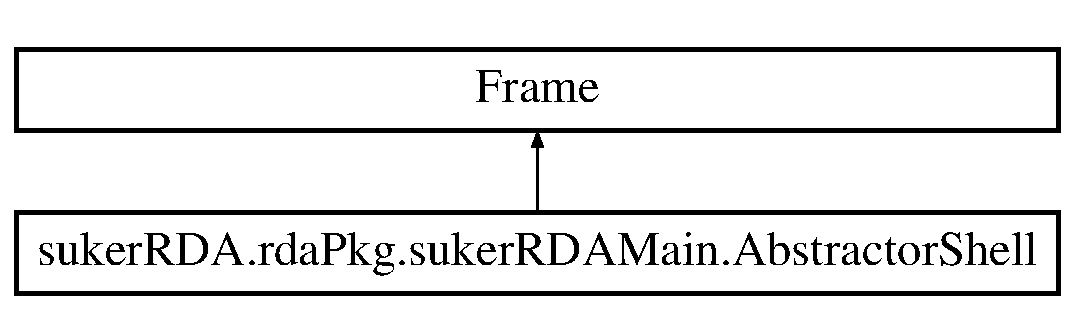
\includegraphics[height=2.000000cm]{classsuker_r_d_a_1_1rda_pkg_1_1suker_r_d_a_main_1_1_abstractor_shell}
\end{center}
\end{figure}
\subsection*{Public Member Functions}
\begin{DoxyCompactItemize}
\item 
\hypertarget{classsuker_r_d_a_1_1rda_pkg_1_1suker_r_d_a_main_1_1_abstractor_shell_aeb1fd1221bd818d3814d8598c44a4dc8}{def {\bfseries \+\_\+\+\_\+init\+\_\+\+\_\+}}\label{classsuker_r_d_a_1_1rda_pkg_1_1suker_r_d_a_main_1_1_abstractor_shell_aeb1fd1221bd818d3814d8598c44a4dc8}

\item 
\hypertarget{classsuker_r_d_a_1_1rda_pkg_1_1suker_r_d_a_main_1_1_abstractor_shell_a659a644e742788468d6f0b60f035f2e2}{def {\bfseries On\+Menu\+File\+Exit}}\label{classsuker_r_d_a_1_1rda_pkg_1_1suker_r_d_a_main_1_1_abstractor_shell_a659a644e742788468d6f0b60f035f2e2}

\item 
\hypertarget{classsuker_r_d_a_1_1rda_pkg_1_1suker_r_d_a_main_1_1_abstractor_shell_a46fb525b28eb6afb6ef21d2c5626cea9}{def {\bfseries On\+Menu\+Help\+About}}\label{classsuker_r_d_a_1_1rda_pkg_1_1suker_r_d_a_main_1_1_abstractor_shell_a46fb525b28eb6afb6ef21d2c5626cea9}

\item 
\hypertarget{classsuker_r_d_a_1_1rda_pkg_1_1suker_r_d_a_main_1_1_abstractor_shell_a0b7fe3b401b06d57b638a9efb25a7fdb}{def {\bfseries On\+Set\+Path}}\label{classsuker_r_d_a_1_1rda_pkg_1_1suker_r_d_a_main_1_1_abstractor_shell_a0b7fe3b401b06d57b638a9efb25a7fdb}

\item 
\hypertarget{classsuker_r_d_a_1_1rda_pkg_1_1suker_r_d_a_main_1_1_abstractor_shell_a9a6c9f91515251d8d27fd6e9c64ab924}{def {\bfseries On\+Radio\+Select}}\label{classsuker_r_d_a_1_1rda_pkg_1_1suker_r_d_a_main_1_1_abstractor_shell_a9a6c9f91515251d8d27fd6e9c64ab924}

\item 
\hypertarget{classsuker_r_d_a_1_1rda_pkg_1_1suker_r_d_a_main_1_1_abstractor_shell_a8ad2057a7f5856cabf0719e3c6824097}{def {\bfseries On\+Parsing}}\label{classsuker_r_d_a_1_1rda_pkg_1_1suker_r_d_a_main_1_1_abstractor_shell_a8ad2057a7f5856cabf0719e3c6824097}

\item 
\hypertarget{classsuker_r_d_a_1_1rda_pkg_1_1suker_r_d_a_main_1_1_abstractor_shell_ad9243ebc32b05f96d209ff780b523b57}{def {\bfseries On\+Open\+Folder}}\label{classsuker_r_d_a_1_1rda_pkg_1_1suker_r_d_a_main_1_1_abstractor_shell_ad9243ebc32b05f96d209ff780b523b57}

\end{DoxyCompactItemize}
\subsection*{Public Attributes}
\begin{DoxyCompactItemize}
\item 
\hypertarget{classsuker_r_d_a_1_1rda_pkg_1_1suker_r_d_a_main_1_1_abstractor_shell_a8b32b6706dcccb849956f08a2a8e0790}{{\bfseries abstractor\+Body\+Cls}}\label{classsuker_r_d_a_1_1rda_pkg_1_1suker_r_d_a_main_1_1_abstractor_shell_a8b32b6706dcccb849956f08a2a8e0790}

\item 
\hypertarget{classsuker_r_d_a_1_1rda_pkg_1_1suker_r_d_a_main_1_1_abstractor_shell_a5060058ec2b699f7ff7dbb54717a9a3e}{{\bfseries logout\+Cls}}\label{classsuker_r_d_a_1_1rda_pkg_1_1suker_r_d_a_main_1_1_abstractor_shell_a5060058ec2b699f7ff7dbb54717a9a3e}

\item 
\hypertarget{classsuker_r_d_a_1_1rda_pkg_1_1suker_r_d_a_main_1_1_abstractor_shell_a0da2823c93dd471e32512533630a09bb}{{\bfseries frame\+\_\+menubar}}\label{classsuker_r_d_a_1_1rda_pkg_1_1suker_r_d_a_main_1_1_abstractor_shell_a0da2823c93dd471e32512533630a09bb}

\item 
\hypertarget{classsuker_r_d_a_1_1rda_pkg_1_1suker_r_d_a_main_1_1_abstractor_shell_a195bc43b4c3bcc348a0a0b290be86619}{{\bfseries wxglade\+\_\+tmp\+\_\+menu}}\label{classsuker_r_d_a_1_1rda_pkg_1_1suker_r_d_a_main_1_1_abstractor_shell_a195bc43b4c3bcc348a0a0b290be86619}

\item 
\hypertarget{classsuker_r_d_a_1_1rda_pkg_1_1suker_r_d_a_main_1_1_abstractor_shell_a6882ea6068474a42025bbf46e5713c1a}{{\bfseries menu\+\_\+file\+\_\+exit}}\label{classsuker_r_d_a_1_1rda_pkg_1_1suker_r_d_a_main_1_1_abstractor_shell_a6882ea6068474a42025bbf46e5713c1a}

\item 
\hypertarget{classsuker_r_d_a_1_1rda_pkg_1_1suker_r_d_a_main_1_1_abstractor_shell_ac2521e9b28dbce7ed1478db12f0c6b7e}{{\bfseries menu\+\_\+help\+\_\+about}}\label{classsuker_r_d_a_1_1rda_pkg_1_1suker_r_d_a_main_1_1_abstractor_shell_ac2521e9b28dbce7ed1478db12f0c6b7e}

\item 
\hypertarget{classsuker_r_d_a_1_1rda_pkg_1_1suker_r_d_a_main_1_1_abstractor_shell_a8eee6f526be88dfc4eb553f23d32d59c}{{\bfseries frame\+\_\+statusbar}}\label{classsuker_r_d_a_1_1rda_pkg_1_1suker_r_d_a_main_1_1_abstractor_shell_a8eee6f526be88dfc4eb553f23d32d59c}

\item 
\hypertarget{classsuker_r_d_a_1_1rda_pkg_1_1suker_r_d_a_main_1_1_abstractor_shell_a9e6b618e9daaf5c103f6139d1737bd7d}{{\bfseries label\+\_\+\+Ram\+Dump\+Path}}\label{classsuker_r_d_a_1_1rda_pkg_1_1suker_r_d_a_main_1_1_abstractor_shell_a9e6b618e9daaf5c103f6139d1737bd7d}

\item 
\hypertarget{classsuker_r_d_a_1_1rda_pkg_1_1suker_r_d_a_main_1_1_abstractor_shell_ae1235d864c80709c8924337b6b0d1155}{{\bfseries text\+\_\+ctrl\+\_\+\+Ram\+Dump\+Path}}\label{classsuker_r_d_a_1_1rda_pkg_1_1suker_r_d_a_main_1_1_abstractor_shell_ae1235d864c80709c8924337b6b0d1155}

\item 
\hypertarget{classsuker_r_d_a_1_1rda_pkg_1_1suker_r_d_a_main_1_1_abstractor_shell_af5f8a647bdaa6673ec71304a53164dea}{{\bfseries label\+\_\+upper\+\_\+right\+\_\+empty}}\label{classsuker_r_d_a_1_1rda_pkg_1_1suker_r_d_a_main_1_1_abstractor_shell_af5f8a647bdaa6673ec71304a53164dea}

\item 
\hypertarget{classsuker_r_d_a_1_1rda_pkg_1_1suker_r_d_a_main_1_1_abstractor_shell_a51f1dca4ba7551b6bcc8f331bf8ed721}{{\bfseries button\+\_\+\+Ram\+Dump\+Path}}\label{classsuker_r_d_a_1_1rda_pkg_1_1suker_r_d_a_main_1_1_abstractor_shell_a51f1dca4ba7551b6bcc8f331bf8ed721}

\item 
\hypertarget{classsuker_r_d_a_1_1rda_pkg_1_1suker_r_d_a_main_1_1_abstractor_shell_a48c863957ac6b767da4fb2ba12a271a4}{{\bfseries text\+\_\+ctrl\+\_\+logs}}\label{classsuker_r_d_a_1_1rda_pkg_1_1suker_r_d_a_main_1_1_abstractor_shell_a48c863957ac6b767da4fb2ba12a271a4}

\item 
\hypertarget{classsuker_r_d_a_1_1rda_pkg_1_1suker_r_d_a_main_1_1_abstractor_shell_a7debc309fe0fc25e35c3f00c3d0e77a9}{{\bfseries radio\+\_\+box\+\_\+crash\+Type}}\label{classsuker_r_d_a_1_1rda_pkg_1_1suker_r_d_a_main_1_1_abstractor_shell_a7debc309fe0fc25e35c3f00c3d0e77a9}

\item 
\hypertarget{classsuker_r_d_a_1_1rda_pkg_1_1suker_r_d_a_main_1_1_abstractor_shell_ac9a3750c3c57a9d4e80a8ba0cdcecb85}{{\bfseries text\+\_\+ctrl\+\_\+log\+\_\+status}}\label{classsuker_r_d_a_1_1rda_pkg_1_1suker_r_d_a_main_1_1_abstractor_shell_ac9a3750c3c57a9d4e80a8ba0cdcecb85}

\item 
\hypertarget{classsuker_r_d_a_1_1rda_pkg_1_1suker_r_d_a_main_1_1_abstractor_shell_aee009ba8fbf4b97c24df9d5016d49dc5}{{\bfseries label\+\_\+1}}\label{classsuker_r_d_a_1_1rda_pkg_1_1suker_r_d_a_main_1_1_abstractor_shell_aee009ba8fbf4b97c24df9d5016d49dc5}

\item 
\hypertarget{classsuker_r_d_a_1_1rda_pkg_1_1suker_r_d_a_main_1_1_abstractor_shell_a4b56219846b415ba92516b291e57ce3c}{{\bfseries text\+\_\+ctrl\+\_\+log\+Size}}\label{classsuker_r_d_a_1_1rda_pkg_1_1suker_r_d_a_main_1_1_abstractor_shell_a4b56219846b415ba92516b291e57ce3c}

\item 
\hypertarget{classsuker_r_d_a_1_1rda_pkg_1_1suker_r_d_a_main_1_1_abstractor_shell_a1a4dad51648de69198b77ef6a06ab8c5}{{\bfseries button\+\_\+\+Run}}\label{classsuker_r_d_a_1_1rda_pkg_1_1suker_r_d_a_main_1_1_abstractor_shell_a1a4dad51648de69198b77ef6a06ab8c5}

\item 
\hypertarget{classsuker_r_d_a_1_1rda_pkg_1_1suker_r_d_a_main_1_1_abstractor_shell_a718a9f8cefa5dbad1fabea2cea3a3040}{{\bfseries button\+\_\+\+Open\+Dir}}\label{classsuker_r_d_a_1_1rda_pkg_1_1suker_r_d_a_main_1_1_abstractor_shell_a718a9f8cefa5dbad1fabea2cea3a3040}

\item 
\hypertarget{classsuker_r_d_a_1_1rda_pkg_1_1suker_r_d_a_main_1_1_abstractor_shell_a06dabc97dc95731a79ac4300aac60995}{{\bfseries label\+\_\+lower\+\_\+empty1}}\label{classsuker_r_d_a_1_1rda_pkg_1_1suker_r_d_a_main_1_1_abstractor_shell_a06dabc97dc95731a79ac4300aac60995}

\item 
\hypertarget{classsuker_r_d_a_1_1rda_pkg_1_1suker_r_d_a_main_1_1_abstractor_shell_a2f194c2a5557993f68f7ed4124f4a78f}{{\bfseries label\+\_\+lower\+\_\+suker\+Mark}}\label{classsuker_r_d_a_1_1rda_pkg_1_1suker_r_d_a_main_1_1_abstractor_shell_a2f194c2a5557993f68f7ed4124f4a78f}

\item 
\hypertarget{classsuker_r_d_a_1_1rda_pkg_1_1suker_r_d_a_main_1_1_abstractor_shell_a3dea7ab58910f24610c20fd714047b21}{{\bfseries dir\+Path}}\label{classsuker_r_d_a_1_1rda_pkg_1_1suker_r_d_a_main_1_1_abstractor_shell_a3dea7ab58910f24610c20fd714047b21}

\end{DoxyCompactItemize}
\subsection*{Static Public Attributes}
\begin{DoxyCompactItemize}
\item 
\hypertarget{classsuker_r_d_a_1_1rda_pkg_1_1suker_r_d_a_main_1_1_abstractor_shell_a7ec1a696336313b5b3234ff0d481af8d}{int {\bfseries abstractor\+Body\+Cls} = 0}\label{classsuker_r_d_a_1_1rda_pkg_1_1suker_r_d_a_main_1_1_abstractor_shell_a7ec1a696336313b5b3234ff0d481af8d}

\item 
\hypertarget{classsuker_r_d_a_1_1rda_pkg_1_1suker_r_d_a_main_1_1_abstractor_shell_ac8e935bd498b6656b2c8b75e2bc6c0ee}{int {\bfseries logout\+Cls} = 0}\label{classsuker_r_d_a_1_1rda_pkg_1_1suker_r_d_a_main_1_1_abstractor_shell_ac8e935bd498b6656b2c8b75e2bc6c0ee}

\item 
\hypertarget{classsuker_r_d_a_1_1rda_pkg_1_1suker_r_d_a_main_1_1_abstractor_shell_acd01df8fa12904ff3dfa81c88df602ad}{string {\bfseries dir\+Path} = \char`\"{}\char`\"{}}\label{classsuker_r_d_a_1_1rda_pkg_1_1suker_r_d_a_main_1_1_abstractor_shell_acd01df8fa12904ff3dfa81c88df602ad}

\end{DoxyCompactItemize}


The documentation for this class was generated from the following file\+:\begin{DoxyCompactItemize}
\item 
suker\+R\+D\+A\+Main.\+py\end{DoxyCompactItemize}

\hypertarget{classsuker_r_d_a_1_1rda_pkg_1_1suker_r_d_a_help_1_1_help_about_dialog}{\section{suker\+R\+D\+A.\+rda\+Pkg.\+suker\+R\+D\+A\+Help.\+Help\+About\+Dialog Class Reference}
\label{classsuker_r_d_a_1_1rda_pkg_1_1suker_r_d_a_help_1_1_help_about_dialog}\index{suker\+R\+D\+A.\+rda\+Pkg.\+suker\+R\+D\+A\+Help.\+Help\+About\+Dialog@{suker\+R\+D\+A.\+rda\+Pkg.\+suker\+R\+D\+A\+Help.\+Help\+About\+Dialog}}
}
Inheritance diagram for suker\+R\+D\+A.\+rda\+Pkg.\+suker\+R\+D\+A\+Help.\+Help\+About\+Dialog\+:\begin{figure}[H]
\begin{center}
\leavevmode
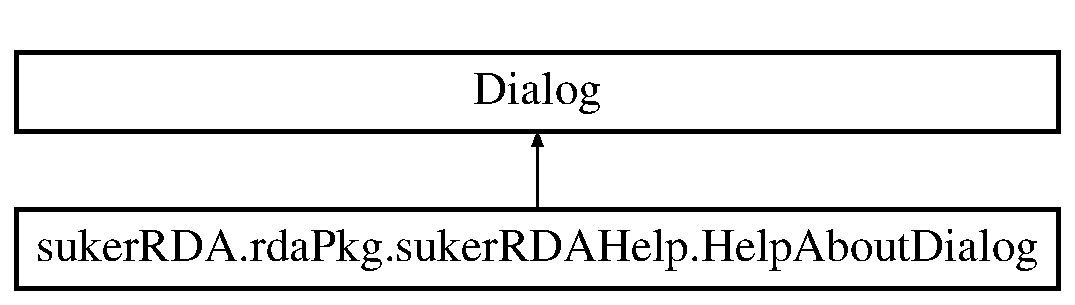
\includegraphics[height=2.000000cm]{classsuker_r_d_a_1_1rda_pkg_1_1suker_r_d_a_help_1_1_help_about_dialog}
\end{center}
\end{figure}
\subsection*{Public Member Functions}
\begin{DoxyCompactItemize}
\item 
\hypertarget{classsuker_r_d_a_1_1rda_pkg_1_1suker_r_d_a_help_1_1_help_about_dialog_aca70ccdf0f4ca44bf502f42d489da61c}{def {\bfseries \+\_\+\+\_\+init\+\_\+\+\_\+}}\label{classsuker_r_d_a_1_1rda_pkg_1_1suker_r_d_a_help_1_1_help_about_dialog_aca70ccdf0f4ca44bf502f42d489da61c}

\end{DoxyCompactItemize}
\subsection*{Public Attributes}
\begin{DoxyCompactItemize}
\item 
\hypertarget{classsuker_r_d_a_1_1rda_pkg_1_1suker_r_d_a_help_1_1_help_about_dialog_a17150991e836c30e2708d014bdf86689}{{\bfseries label\+\_\+about\+\_\+empty1}}\label{classsuker_r_d_a_1_1rda_pkg_1_1suker_r_d_a_help_1_1_help_about_dialog_a17150991e836c30e2708d014bdf86689}

\item 
\hypertarget{classsuker_r_d_a_1_1rda_pkg_1_1suker_r_d_a_help_1_1_help_about_dialog_aa83891e2d04184db0aa734f2a88c733c}{{\bfseries bitmap\+\_\+1}}\label{classsuker_r_d_a_1_1rda_pkg_1_1suker_r_d_a_help_1_1_help_about_dialog_aa83891e2d04184db0aa734f2a88c733c}

\item 
\hypertarget{classsuker_r_d_a_1_1rda_pkg_1_1suker_r_d_a_help_1_1_help_about_dialog_a585acecefe8e3705ce89e788faf3d4b1}{{\bfseries label\+\_\+using\+Explain}}\label{classsuker_r_d_a_1_1rda_pkg_1_1suker_r_d_a_help_1_1_help_about_dialog_a585acecefe8e3705ce89e788faf3d4b1}

\item 
\hypertarget{classsuker_r_d_a_1_1rda_pkg_1_1suker_r_d_a_help_1_1_help_about_dialog_aeedc31b05cdbf3788d3452d4b55d5e69}{{\bfseries label\+\_\+using\+About\+Me}}\label{classsuker_r_d_a_1_1rda_pkg_1_1suker_r_d_a_help_1_1_help_about_dialog_aeedc31b05cdbf3788d3452d4b55d5e69}

\end{DoxyCompactItemize}


The documentation for this class was generated from the following file\+:\begin{DoxyCompactItemize}
\item 
suker\+R\+D\+A\+Help.\+py\end{DoxyCompactItemize}

\hypertarget{classsuker_r_d_a_1_1rda_pkg_1_1suker_r_d_a_log_out_1_1log_outputs}{\section{suker\+R\+D\+A.\+rda\+Pkg.\+suker\+R\+D\+A\+Log\+Out.\+log\+Outputs Class Reference}
\label{classsuker_r_d_a_1_1rda_pkg_1_1suker_r_d_a_log_out_1_1log_outputs}\index{suker\+R\+D\+A.\+rda\+Pkg.\+suker\+R\+D\+A\+Log\+Out.\+log\+Outputs@{suker\+R\+D\+A.\+rda\+Pkg.\+suker\+R\+D\+A\+Log\+Out.\+log\+Outputs}}
}
\subsection*{Public Member Functions}
\begin{DoxyCompactItemize}
\item 
\hypertarget{classsuker_r_d_a_1_1rda_pkg_1_1suker_r_d_a_log_out_1_1log_outputs_a4ac0f6ac65e8c375169666b884d35011}{def {\bfseries \+\_\+\+\_\+init\+\_\+\+\_\+}}\label{classsuker_r_d_a_1_1rda_pkg_1_1suker_r_d_a_log_out_1_1log_outputs_a4ac0f6ac65e8c375169666b884d35011}

\item 
\hypertarget{classsuker_r_d_a_1_1rda_pkg_1_1suker_r_d_a_log_out_1_1log_outputs_a8cab869939222e567a521d54ebf73876}{def {\bfseries lk\+Write\+Outs}}\label{classsuker_r_d_a_1_1rda_pkg_1_1suker_r_d_a_log_out_1_1log_outputs_a8cab869939222e567a521d54ebf73876}

\item 
\hypertarget{classsuker_r_d_a_1_1rda_pkg_1_1suker_r_d_a_log_out_1_1log_outputs_ae3bb69a6f5987f65f6fde057fc440be9}{def {\bfseries kernel\+Write\+Outs}}\label{classsuker_r_d_a_1_1rda_pkg_1_1suker_r_d_a_log_out_1_1log_outputs_ae3bb69a6f5987f65f6fde057fc440be9}

\item 
\hypertarget{classsuker_r_d_a_1_1rda_pkg_1_1suker_r_d_a_log_out_1_1log_outputs_a18f5192325b6db0d383fbe03291b00fe}{def {\bfseries etc\+Write\+Outs}}\label{classsuker_r_d_a_1_1rda_pkg_1_1suker_r_d_a_log_out_1_1log_outputs_a18f5192325b6db0d383fbe03291b00fe}

\item 
\hypertarget{classsuker_r_d_a_1_1rda_pkg_1_1suker_r_d_a_log_out_1_1log_outputs_a43fd092a3322c49e7d0c988cfc6c1121}{def {\bfseries get\+L\+K\+Outs}}\label{classsuker_r_d_a_1_1rda_pkg_1_1suker_r_d_a_log_out_1_1log_outputs_a43fd092a3322c49e7d0c988cfc6c1121}

\item 
\hypertarget{classsuker_r_d_a_1_1rda_pkg_1_1suker_r_d_a_log_out_1_1log_outputs_a04eb793b5fa2732357b64805f4e67654}{def {\bfseries get\+Kernel\+Outs}}\label{classsuker_r_d_a_1_1rda_pkg_1_1suker_r_d_a_log_out_1_1log_outputs_a04eb793b5fa2732357b64805f4e67654}

\item 
\hypertarget{classsuker_r_d_a_1_1rda_pkg_1_1suker_r_d_a_log_out_1_1log_outputs_aa2c5ec19cf75b5af6e2133384e25dfef}{def {\bfseries get\+Etc\+Outs}}\label{classsuker_r_d_a_1_1rda_pkg_1_1suker_r_d_a_log_out_1_1log_outputs_aa2c5ec19cf75b5af6e2133384e25dfef}

\item 
\hypertarget{classsuker_r_d_a_1_1rda_pkg_1_1suker_r_d_a_log_out_1_1log_outputs_a7f2e3fcfd4f44a2e234bb743efe87a81}{def {\bfseries all\+Clear\+List}}\label{classsuker_r_d_a_1_1rda_pkg_1_1suker_r_d_a_log_out_1_1log_outputs_a7f2e3fcfd4f44a2e234bb743efe87a81}

\end{DoxyCompactItemize}
\subsection*{Public Attributes}
\begin{DoxyCompactItemize}
\item 
\hypertarget{classsuker_r_d_a_1_1rda_pkg_1_1suker_r_d_a_log_out_1_1log_outputs_a8d4d58d39ce0c1b0d420ef5cd3e57652}{{\bfseries lk\+Out}}\label{classsuker_r_d_a_1_1rda_pkg_1_1suker_r_d_a_log_out_1_1log_outputs_a8d4d58d39ce0c1b0d420ef5cd3e57652}

\item 
\hypertarget{classsuker_r_d_a_1_1rda_pkg_1_1suker_r_d_a_log_out_1_1log_outputs_a9d387790f667307a0b391fd157ffa657}{{\bfseries kernel\+Out}}\label{classsuker_r_d_a_1_1rda_pkg_1_1suker_r_d_a_log_out_1_1log_outputs_a9d387790f667307a0b391fd157ffa657}

\item 
\hypertarget{classsuker_r_d_a_1_1rda_pkg_1_1suker_r_d_a_log_out_1_1log_outputs_aeef61f468eed55ce60e8c9b2a2f52f47}{{\bfseries etc\+Out}}\label{classsuker_r_d_a_1_1rda_pkg_1_1suker_r_d_a_log_out_1_1log_outputs_aeef61f468eed55ce60e8c9b2a2f52f47}

\end{DoxyCompactItemize}
\subsection*{Static Public Attributes}
\begin{DoxyCompactItemize}
\item 
\hypertarget{classsuker_r_d_a_1_1rda_pkg_1_1suker_r_d_a_log_out_1_1log_outputs_a3b3a18e0090db0e77ec41ff62e137628}{list {\bfseries lk\+Out} = \mbox{[}$\,$\mbox{]}}\label{classsuker_r_d_a_1_1rda_pkg_1_1suker_r_d_a_log_out_1_1log_outputs_a3b3a18e0090db0e77ec41ff62e137628}

\item 
\hypertarget{classsuker_r_d_a_1_1rda_pkg_1_1suker_r_d_a_log_out_1_1log_outputs_a9616068e8e486c69111305b39e711b5a}{list {\bfseries kernel\+Out} = \mbox{[}$\,$\mbox{]}}\label{classsuker_r_d_a_1_1rda_pkg_1_1suker_r_d_a_log_out_1_1log_outputs_a9616068e8e486c69111305b39e711b5a}

\item 
\hypertarget{classsuker_r_d_a_1_1rda_pkg_1_1suker_r_d_a_log_out_1_1log_outputs_af3acdc343ffe0cbdd9565f60d18b1f6a}{list {\bfseries etc\+Out} = \mbox{[}$\,$\mbox{]}}\label{classsuker_r_d_a_1_1rda_pkg_1_1suker_r_d_a_log_out_1_1log_outputs_af3acdc343ffe0cbdd9565f60d18b1f6a}

\end{DoxyCompactItemize}


The documentation for this class was generated from the following file\+:\begin{DoxyCompactItemize}
\item 
suker\+R\+D\+A\+Log\+Out.\+py\end{DoxyCompactItemize}

%--- End generated contents ---

% Index
\newpage
\phantomsection
\addcontentsline{toc}{chapter}{Index}
\printindex

\end{document}
